\documentclass[12pt,aspectratio=43]{beamer}

%%%%%%%%%%%%%%%%%%%%%%%%%%%%%%%%%%%%%%%%
% Paquetes de configuración basica del %
%               texto                  %
%%%%%%%%%%%%%%%%%%%%%%%%%%%%%%%%%%%%%%%%
\usepackage[spanish,es-nodecimaldot]{babel}
\usepackage[T1]{fontenc}
\usepackage{listings}
\usepackage{hyperref}
\usepackage{ifthen}

%%%%%%%%%%%%%%%%%%%%%%%%%%%%%%%%%%%%%%%%%%%%%
% [listings] Configuración de vizualizacion %
% de código                                 %
%%%%%%%%%%%%%%%%%%%%%%%%%%%%%%%%%%%%%%%%%%%%%
\lstset{
	basicstyle=\ttfamily,
	extendedchars=true,
	showspaces=false,
	showstringspaces=false,
	captionpos=b,
	keywordstyle=\bfseries\color{cyan},
	commentstyle=\color{gray},
	stringstyle=\color{orange},
	escapeinside={!>}{<!} }

%%%%%%%%%%%%%%%%%%%%%%%%%%%%%%%%%%%%%%%%
%  Paquetes de configuración graficos  %
%            del documento             %
%%%%%%%%%%%%%%%%%%%%%%%%%%%%%%%%%%%%%%%%
\usepackage{graphicx}
\usepackage{tikz}
\usetikzlibrary{babel}
\usepackage{xcolor}
\usepackage{pdfpages}
\usepackage{animate}

\usepackage{ifxetex}
\ifxetex
	\usepackage[no-math]{fontspec}
	\setmainfont{AncizarSans}[
		Path = ../Fuentes/,
		Extension = .otf,
		BoldFont = *-B,
		ItalicFont = *-I,
		BoldItalicFont = *-BI ]
	\setmonofont{UbuntuMono}[
		Path = ../Fuentes/,
		Extension = .ttf,
		BoldFont = *-B,
		ItalicFont = *-I,
		BoldItalicFont = *-BI ]
	\newcommand{\lmr}{\fontfamily{lmr}\selectfont}
	\newcommand{\lmss}{\fontfamily{lmss}\selectfont}
	\newcommand{\lmtt}{\fontfamily{lmtt}\selectfont}
\fi

%%%%%%%%%%%%%%%%%%%%%%%%%%%%%%%%%%%%%%%%
%      Configuraciones de Beamer       %
%%%%%%%%%%%%%%%%%%%%%%%%%%%%%%%%%%%%%%%%
\definecolor{Igreen}{RGB}{148,180,59}
\definecolor{Ired}{RGB}{166,24,49}

\setbeamertemplate{navigation symbols}{}

\setbeamertemplate{itemize items}{\color{Igreen}\raisebox{.45ex}{\rule{.6ex}{.6ex}}}

\usefonttheme{professionalfonts}
\usefonttheme{serif}
\setbeamercolor{frametitle}{fg=Ired,bg=Igreen!50}
\setbeamercolor{alerted text}{fg=Ired}

\makeatletter
\newcommand{\ifratio}[2]{
	\ifthenelse
		{\lengthtest{\beamer@paperwidth=16cm} \AND \lengthtest{\beamer@paperheight=9cm}}
		{#1}
		{#2} }
\makeatother

%%%%%%%%%%%%%%%%%%%%%%%%%%%%%%%%%%%%%%%%
%    Información de la presentación    %
%%%%%%%%%%%%%%%%%%%%%%%%%%%%%%%%%%%%%%%%
\title{Introducción a {\lmr\LaTeX}}
\subtitle{Curso Libre de {\lmr\LaTeX}}
\author{Joar Esteban Buitrago Carrillo}
\institute{Universidad Nacional de Colombia}
\date{}
\logo{
\includegraphics[height=0.75cm]{../Escudo_UN}}

\setbeamertemplate{title page}{
	\begin{tikzpicture}[overlay,remember picture]
	\path (current page.north west) ++(0.5cm,-0.5cm) node[below right] {
\includegraphics[height=1.25cm]{../Escudo_UN}};
	\path (current page.north east) ++(-0.5cm,-0.5cm) node[below left] {\parbox[c][1.25cm][c]{\widthof{\Large \insertsubtitle}}{\Large \insertsubtitle}};
	\end{tikzpicture}

	\vfill
	\begin{center}
		{\Huge\inserttitle}\\
		\bigskip
		\insertauthor
	\end{center}
	\vfill
}

\begin{document}
\begin{frame}[plain]
\titlepage
\end{frame}

{
\setbeamercolor{background canvas}{bg=}
\begin{frame}
\ifratio
	{\includepdf[pages=2]{../Licencia_Diapositiva.pdf}}
	{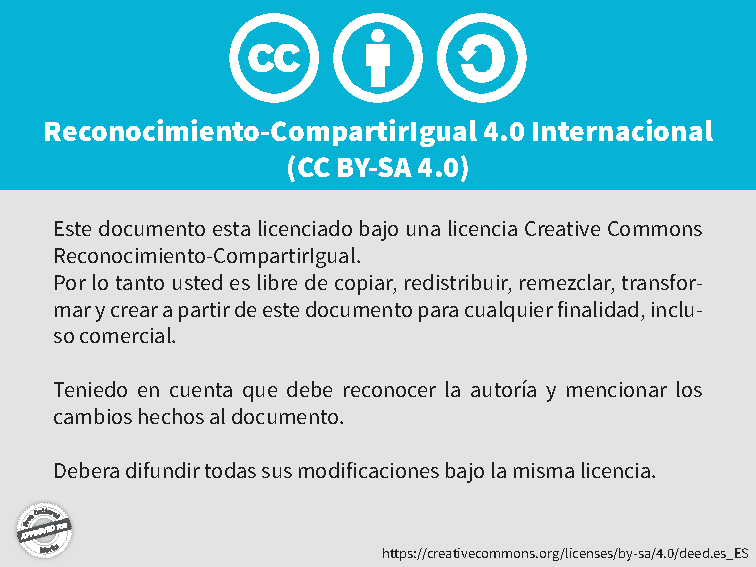
\includepdf[pages=1]{../Licencia_Diapositiva.pdf}}
\end{frame}
}

\begin{frame}{¿Que es {\lmr\LaTeX}?}{}
{\lmr\LaTeX} es un sistema de composición de textos de calidad artística y tipográfica. Es usado muy habitualmente en el mundo científico debido a todas sus características y facilidad de trabajo.\pause\\[2em]

{\lmr\LaTeX} es un conjunto de macros de {\lmr\TeX}, licenciado bajo la licencia {\it{\lmr L}PPL}, {\it{\lmr\LaTeX} Project Public License}. Por lo cual es {\em Software Libre} y gratuito.
\end{frame}

\begin{frame}[fragile]{Funciones Seno y Coseno}
\begin{center}
%	\begin{animateinline}[autoplay,loop,nomouse,poster=first]{24}
%		\multiframe{359}{nAngle=0+1}{
%			\begin{tikzpicture}
%			\draw[thick,-latex,blue] (-3,0) -- (3,0) node[right] {$x$};
%			\draw[thick,-latex,blue] (0,-3) -- (0,3) node[above] {$y$};
%			\draw[red,thick] (0,0) circle (2.5);
%			\draw[ultra thick,cyan] (0,0) -- (0,0 |- \nAngle:2.5) node[midway,left] {$\sin(\alpha)$};
%			\draw[ultra thick,orange] (0,0) -- (\nAngle:2.5 |- 0,0) node[midway,below] {$\cos(\alpha)$};
%			\draw[densely dotted,orange] (\nAngle:2.5) -- (\nAngle:2.5 |- 0,0);
%			\draw[densely dotted,cyan] (\nAngle:2.5) -- (0,0 |- \nAngle:2.5);
%			\draw[thick,green] (0.5,0) arc (0:\nAngle:0.5);
%			\draw[thick,green,opacity=0] (0.7,0) arc (0:\nAngle:0.7) node[midway,opacity=1] {$\alpha$};
%			\draw[ultra thick,red,-latex] (0,0) -- (\nAngle:2.5);
%			\end{tikzpicture}
%		}
%	\end{animateinline}
\end{center}
\end{frame}

\section{Clases}
\begin{frame}{Clases del documento}{}
Al trabajar en un documento escrito con {\lmr\LaTeX} debemos tener en cuenta la clase del documento en el cual queremos trabajar, la clase más usada generalmente es \texttt{\textbf{article}}.\pause\\[2em]

Las clases «estándares» de {\lmr\LaTeX} son:
\begin{itemize}
	\item {\color{Ired}\texttt{article}}: para artículos.
	\item {\color{Ired}\texttt{report}}: para reportes.
	\item {\color{Ired}\texttt{book}}: para libros.
	\item {\color{Ired}\texttt{letter}}: para las cartas.
	\item {\alt<3>{\color{black!30!Igreen}\textbf{\texttt{beamer}}}{\color{Ired} \texttt{slides}}}: para las presentaciones.
\end{itemize}
\end{frame}

\begin{frame}[fragile]{Clases del documento}{}
Para indicar la clase del documento a {\lmr\LaTeX} solo debemos de escribir en nuestro código:
\begin{center}
	\lstinline[language={[LaTeX]TeX}]|\documentclass{<clase>}|
\end{center}
\pause
Donde \texttt{<clase>} es cualquiera de las clases ya mencionadas, u otras personalizadas o descargadas.
\end{frame}

\section{Estructura del código}
\begin{frame}[fragile]{Estructura del código}{}
La estructura básica del código de cualquier documento es muy sencilla, siempre es la misma.

\begin{enumerate}
	\item Primero se coloca el comando \lstinline[language={[LaTeX]TeX}]|\documentclass{<clase>}| con la clase escogida.
	\item Desde aquí encontramos el \alert{\bf preámbulo} hasta que se encuentra la orden \lstinline[language={[LaTeX]TeX}]|\begin{document}|.
	\item Después tenemos el \alert{\bf cuerpo del documento} hasta encontrar la orden \lstinline[language={[LaTeX]TeX}]|\end{document}|, todo lo que se encuentra después de esto es ignorado por {\lmr\LaTeX}.
\end{enumerate}

Se debe tener cuidado al escribir, ya que existen comandos que solo funcionan en una sección del código.
\end{frame}

\begin{frame}[fragile]{Estructura del código}{Código}
De manera más visual esto seria:
\begin{lstlisting}[language={[LaTeX]TeX}]
\documentclass{<clase>}

Preámbulo ...

\begin{document}

Documento ...

\end{document}

Esto puede servir como comentario
Ya que es ignorado ...
\end{lstlisting}
\end{frame}

\section{Títulos}

\section{Capítulos-Partes, Secciones, etc.}

\section{El resumen}

\section{Estilos, Familias y Formas}

\section{Tamaño de fuente}

\section{Paquetes {\tt fontenc} e {\tt inputenc}}

\section{{\lmr\LaTeX} en español}

\section{Separación del texto}

\section{Opciones del Documento}
\end{document}
